\part{Behaviour Trees}
\frame{\partpage}

\begin{frame}{Behaviour trees (BTs)}
	\begin{itemize}
		\pause\item A \textbf{hierarchical} model of decision making
		\pause\item Allow \textbf{complex behaviours} to be built up from \textbf{simple components}
		\pause\item Allow for \textbf{more complex} behaviours than FSMs
		\pause\item First used in Halo 2 (2005), now used extensively
		\pause\item Also used in robotics and other non-game AI applications
	\end{itemize}
\end{frame}

\begin{frame}{Using BTs}
	\begin{itemize}
		\pause\item Fairly easy to implement; plenty of resources online
		\pause\item \textbf{Unreal}: an advanced BT system is built in
		\pause\item \textbf{Unity}: numerous free and paid options on the Asset Store
			e.g.\ Behavior Machine, Behavior Designer, Behave, RAIN
	\end{itemize}
\end{frame}

\begin{frame}{BT basics}
	\begin{itemize}
		\pause\item A BT is a \textbf{tree} of \textbf{nodes}
		\pause\item On each game update (i.e.\ each frame), the root node is \textbf{ticked}
			\begin{itemize}
				\pause\item When a node is ticked, it might cause some or all of its \textbf{children} to tick as well
				\pause\item So ticks propagate down the tree from the root
			\end{itemize}
		\pause\item A ticked node returns one of three \textbf{statuses}:
			\begin{itemize}
				\pause\item Success
				\pause\item Running
				\pause\item Failure
			\end{itemize}
		\pause\item ``Running'' status allows nodes to represent operations that \textbf{last multiple frames}
	\end{itemize}
\end{frame}

\begin{frame}{Blackboard}
	\begin{itemize}
		\pause\item It is often useful to \textbf{share} data between nodes
		\pause\item A \textbf{blackboard} (sometimes called a \textbf{data context}) allows this
		\pause\item Blackboard defines \textbf{variables}, which can be \textbf{read} and \textbf{written} by nodes
		\pause\item Blackboard can be \textbf{local} to the AI agent, \textbf{shared} between several agents, or \textbf{global} to all agents
		\pause\item (Shared blackboards mean that your AI has ``telepathy'' --- this may or may not be desirable!)
	\end{itemize}
\end{frame}

\begin{frame}{BTs in The Division}
	\begin{center}
		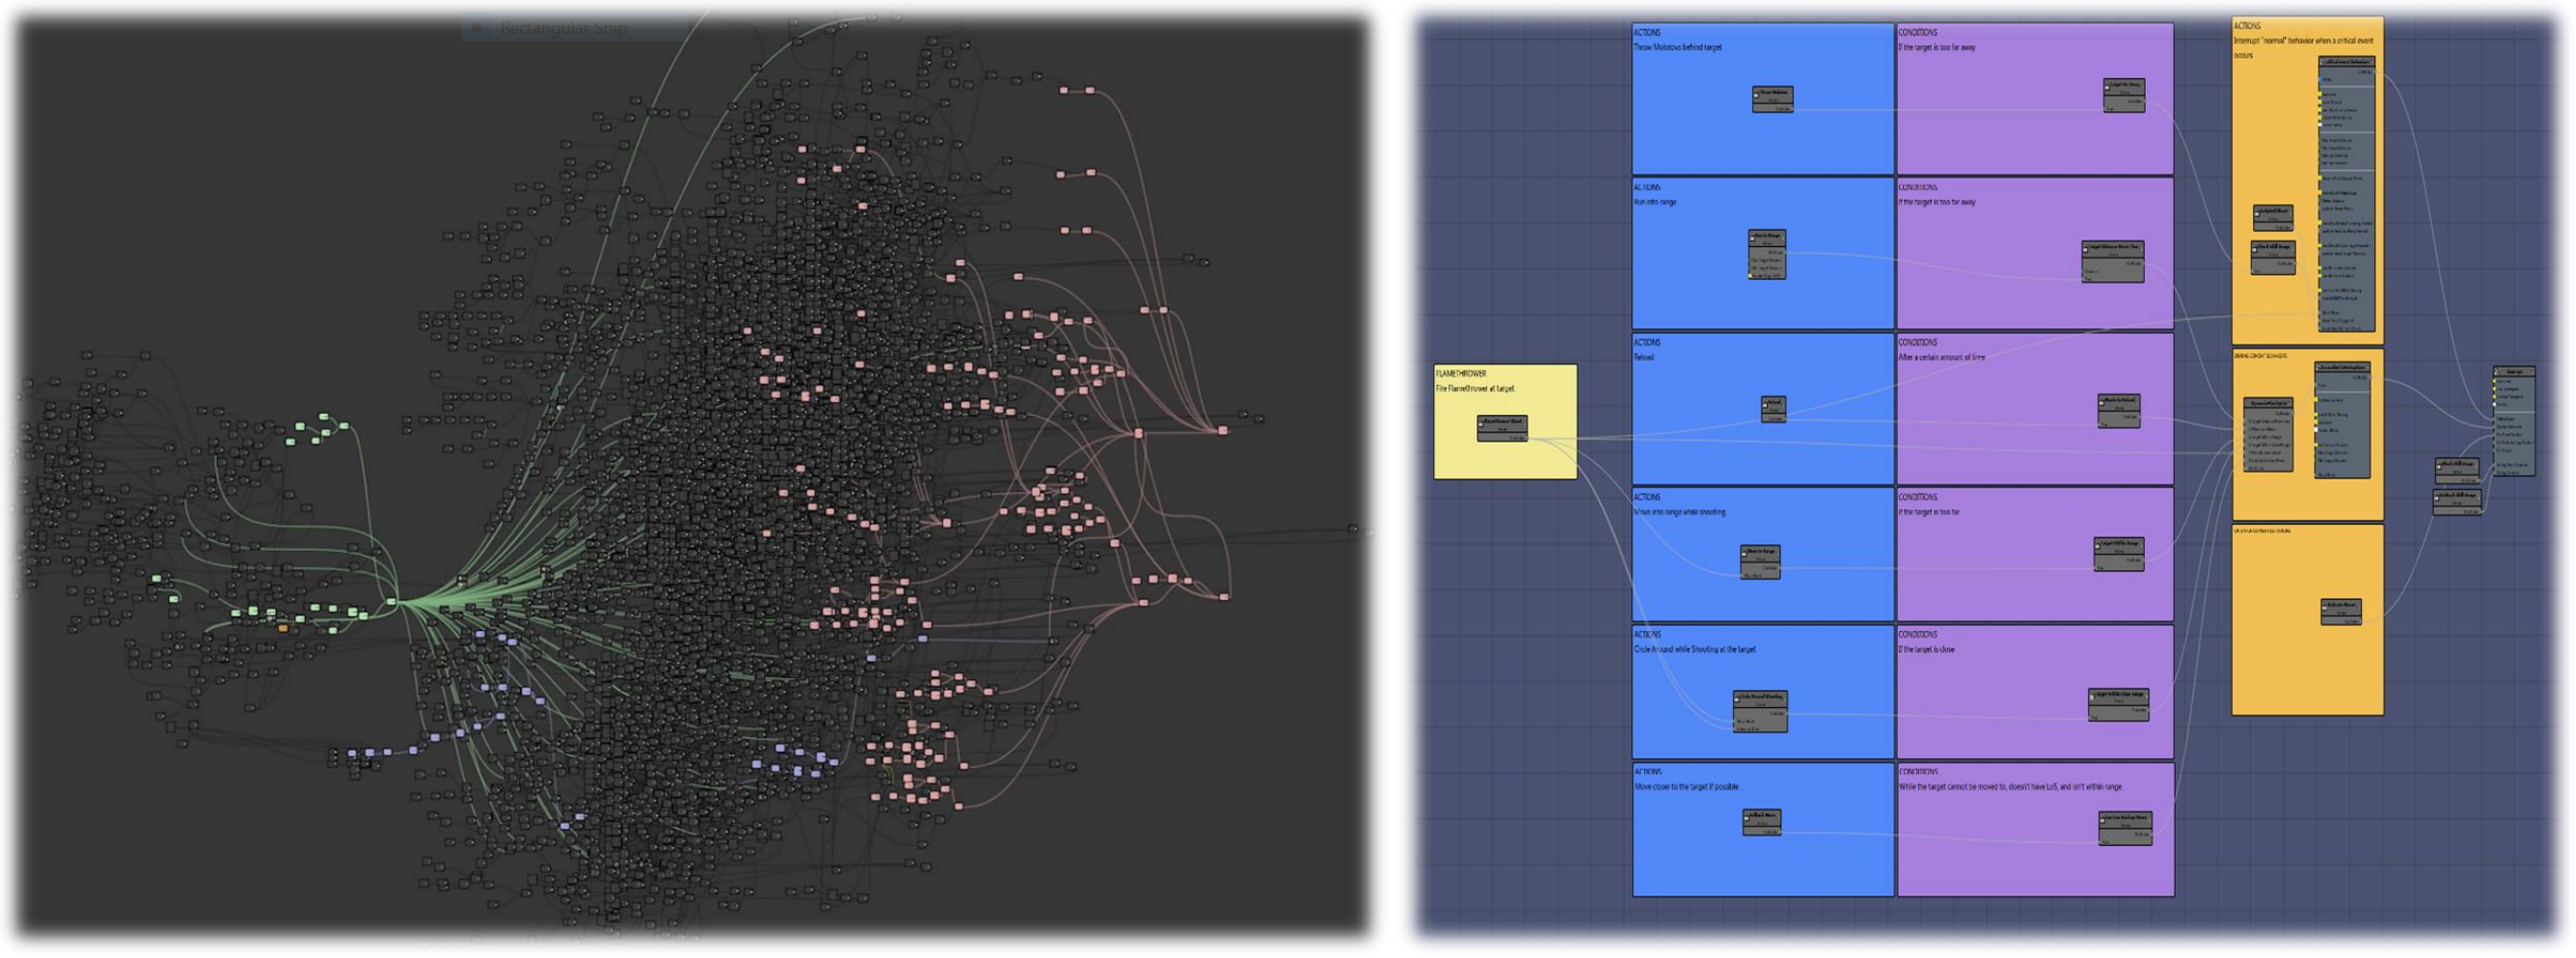
\includegraphics[width=\textwidth]{the_division}
		
		\url{http://www.gdcvault.com/play/1023382/AI-Behavior-Editing-and-Debugging}
	\end{center}
\end{frame}
